
%(BEGIN_QUESTION)
% Copyright 2010, Tony R. Kuphaldt, released under the Creative Commons Attribution License (v 1.0)
% This means you may do almost anything with this work of mine, so long as you give me proper credit

This room pressure control system maintains a slightly positive pressure in a precision electronic assembly room to prevent dust from entering from the outside, while always ensuring a rapid flow rate of air through the room.  It regulates pressure by modulating two variable-speed fans: one introducing air to the room (the ``forced draft'' fan) and one venting air from the room (the ``induced draft'' fan).  A pressure transmitter outputs 4 mA at 0 "W.C room pressure and 20 mA at 2 "W.C. room pressure:
 
$$\includegraphics[width=15.5cm]{i01566x01.eps}$$

Suppose you are called to troubleshoot a problem in this system: the room air pressure is holding steady at +0.17 inches WC (according to the display on the DDC control system) with the FD fan running at 100\% speed and the ID fan running at 0\% speed.  Based on this data, identify the most likely cause of the problem, and also how you would confirm your diagnosis {\it before} making any repairs.

\vskip 10pt

Next, calculate the amount of force exerted on a walk-in door from the room's positive pressure (at setpoint) assuming the door is 30 inches wide and 84 inches tall.

\vskip 20pt \vbox{\hrule \hbox{\strut \vrule{} {\bf Suggestions for Socratic discussion} \vrule} \hrule}

\begin{itemize}
\item{} What does ``VFD'' stand for, and what exactly do the ``VFD'' boxes do to exert control over the speed of the two fan motors?
\item{} Determine the most likely combination of split-ranges for the two controller outputs (0 to 10 volts DC each, with each VFD calibrated for 0\% speed at 0 volts and 100\% speed at 10 volts).
\item{} Determine the effect a failed PT (high output signal) will have on room pressure.
\item{} Determine the effect a failed FD VFD (motor dead) will have on room pressure.
\item{} Determine the effect a failed ID VFD (motor dead) will have on room pressure.
\end{itemize}

\underbar{file i01566}
%(END_QUESTION)





%(BEGIN_ANSWER)

One possibility here is that the air filter is plugged.

%(END_ANSWER)





%(BEGIN_NOTES)

Other possibilities include a large air leak in the room (e.g. window or large door left open), or a fault in the transmitter causing it to read much too low.

\vskip 10pt

Monitor the differential pressure across the air filter to see whether or not it is excessive.  If so, the filter is clogged.  If not, the problem is more likely a leak in the room.  A simple way to monitor air pressure is to use a water manometer to measure the pressure difference inside and out.

\vskip 10pt

The pressure differential across the walk-in door (at setpoint is 0.25 inches water column, or 0.009032 PSI).  The door has a surface area equal to its height times its width ($A$ = 30 inches $\times$ 84 inches = 2520 square inches).  Since force is equal to pressure times area ($F = PA$), the force exerted on this door by the differential pressure will be:

$$F = PA$$

$$F = (2520 \hbox{ in}^2)(0.009032 \hbox{ lbs/in}^2) = 22.76 \hbox{ lbs}$$











\vskip 20pt \vbox{\hrule \hbox{\strut \vrule{} {\bf Virtual Troubleshooting} \vrule} \hrule}

This question is a good candidate for a ``Virtual Troubleshooting'' exercise.  Presenting the diagram to students, you first imagine in your own mind a particular fault in the system.  Then, you present one or more symptoms of that fault (something noticeable by an operator or other user of the system).  Students then propose various diagnostic tests to perform on this system to identify the nature and location of the fault, as though they were technicians trying to troubleshoot the problem.  Your job is to tell them what the result(s) would be for each of the proposed diagnostic tests, documenting those results where all the students can see.

During and after the exercise, it is good to ask students follow-up questions such as:

\begin{itemize}
\item{} What does the result of the last diagnostic test tell you about the fault?
\item{} Suppose the results of the last diagnostic test were different.  What then would that result tell you about the fault?
\item{} Is the last diagnostic test the best one we could do?
\item{} What would be the ideal order of tests, to diagnose the problem in as few steps as possible?
\end{itemize}

%INDEX% Process: clean room pressure control

%(END_NOTES)


